\lab{LAB: Arduino Gamecontroller}

\apparatus
\equip{Computer}
\equip{Anaconda}
\equip{Jupyter Notebook}
\equip{VPython (for Jupyter)}
\equip{Arduino IDE programming editor and compiler}
\equip{Arduino Uno microprocessor}
\equip{breadboard}
\equip{2-axis potentiometer (joystick)}
\equip{wiring kit}
\equip{LED}
\equip{pushbutton SPST switch}

\longgoal

The purpose of this activity is to build a game controller and to use the game controller to operate the thruster in the Lunar Lander game. You will install a number of software packages to make this possible. The project requires: (1) biulding 

\procedure

There are four steps:

\begin{enumerate}
	\item Install software
	\item Build the game controller
	\item Upload an Arduino program to the Arduino Uno
	\item Run Lunar Lander with the Arduino game controller
\end{enumerate}

\begin{enumerate}

\subsection*{Install Software}

\item Go to our course web site where you will find links to download and install software.

\item Install the Arduino IDE for writing and compiling Arduino programs and uploading to an Arduino board.

\item Install the Anaconda distribution of the Python 2.7 programming language and scientific packages. {\bf IMPORTANT -- DOWNLOAD THE INSTALLER FOR PYTHON 2.7.} (not Python 3.5)

\item After you install Anaconda, open a terminal window (also called the command line). On a Mac, you will do this by opening Applications$\to$Utilities$\to$Terminal. It should look similar to the following terminal window.

\scaledimage{arduino-gamecontroller/terminal}{Terminal window.}{0.3}

\item To verify that Anaconda is installed property, at the command line, type the following:

\begin{verbatim}
which conda
\end{verbatim}

The command \code{which} returns the filepath to the location of the conda program.

\item Now, type \code{which jupyter} at the command line. It should return the path to the jupyter program as shown in Figure \ref{arduino-gamecontroller/which}.

\scaledimage{arduino-gamecontroller/which}{Terminal window showing path to conda and path to jupyter.}{0.3}


{\bf If this command does not return a path to jupyter, then you need to install Jupyter.}  In this case, type the command:

\begin{verbatim}
conda install jupyter
\end{verbatim}

\item Install the \code{vpython} package by typing:

\begin{verbatim}
pip install vpython
\end{verbatim}

\item Install the \code{pyserial} package by typing:

\begin{verbatim}
pip install pyserial
\end{verbatim}

To test your software installation, we will open a Jupyter Notebook, import vpython and pyserial packages, and create a 3D object. If it is successful and produces no error messages, then we are confident that we will be able to develop programs that use our game controller.

\item At the command line, type

\begin{verbatim}
jupyter notebook
\end{verbatim}

A Jupyter window will open in your web browser showing your files and folders in your home directory (or whatever directory you are in when you launch jupyter notebook), as shown in Figure \ref{arduino-gamecontroller/jupyter}. 

\scaledimage{arduino-gamecontroller/jupyter}{A Jupyter window.}{0.5}

\item You can clink the folder links to navigate to the folder of your choice. Then, create a new notebook by clicking the \frame{\ New\ } button in the Jupyter toolbar. In the menu, select the \code{VPython} notebook, as shown in Figure \ref{arduino-gamecontroller/new}.

\scaledimage{arduino-gamecontroller/new}{Creating a new notebook}{0.5}

This creates a new notebook file as shown in Figure \ref{arduino-gamecontroller/nb}. 

\scaledimage{arduino-gamecontroller/nb}{A newly created Jupyter notebook}{0.3}

\item Click the name ``Untitled'' and change the name to something more appropriate like ``notebook-test'' or something like that. I suggest that you do not use blanks or characters other than a hypen or underscore in filenames.

\item In the first cell, type

\begin{myvpython}
from vpython import *
\end{myvpython}

{\bf Use shift-RETURN to run the code in the cell.}

After running, the cell will receive the number 1 and will be labeled \code{In  [1]:}. The numbering system shows you the sequence that cells were run.

\item In the second cell, type

\begin{myvpython}
from serial import *
\end{myvpython}

Again, use shift-RETURN to run the cell. (Do this for every cell in order to run it.) At this point, there should be no error messages.

\item Now, we have to create a canvas (i.e. scene) and a 3D object. In the third cell, type and run the following code:

\begin{myvpython}
scene=canvas(title="3D scene")
sphere()
\end{myvpython}

You should see a sphere like the example in Figure \ref{arduino-gamecontroller/sphere}.

\scaledimage{arduino-gamecontroller/sphere}{A VPython program running in a Jupyter notebook.}{0.3}

{\bf If you receive any errors up to this point, please get help. This program must work before you continue.}

\subsection*{Build the game controller}

Here are the parts:

\begin{enumerate}
	\item an Arduino Uno microprocessor
	\item a breadboard
	\item a LED
	\item a push button SPST switch
	\item a 1000 $\ohm$ resistor
	\item a Parallax 2-axis joystick
	\item a wiring kit
	\item a USB cable
	\item a rubber band
\end{enumerate}

Here are photos that show the wiring for the game controller.

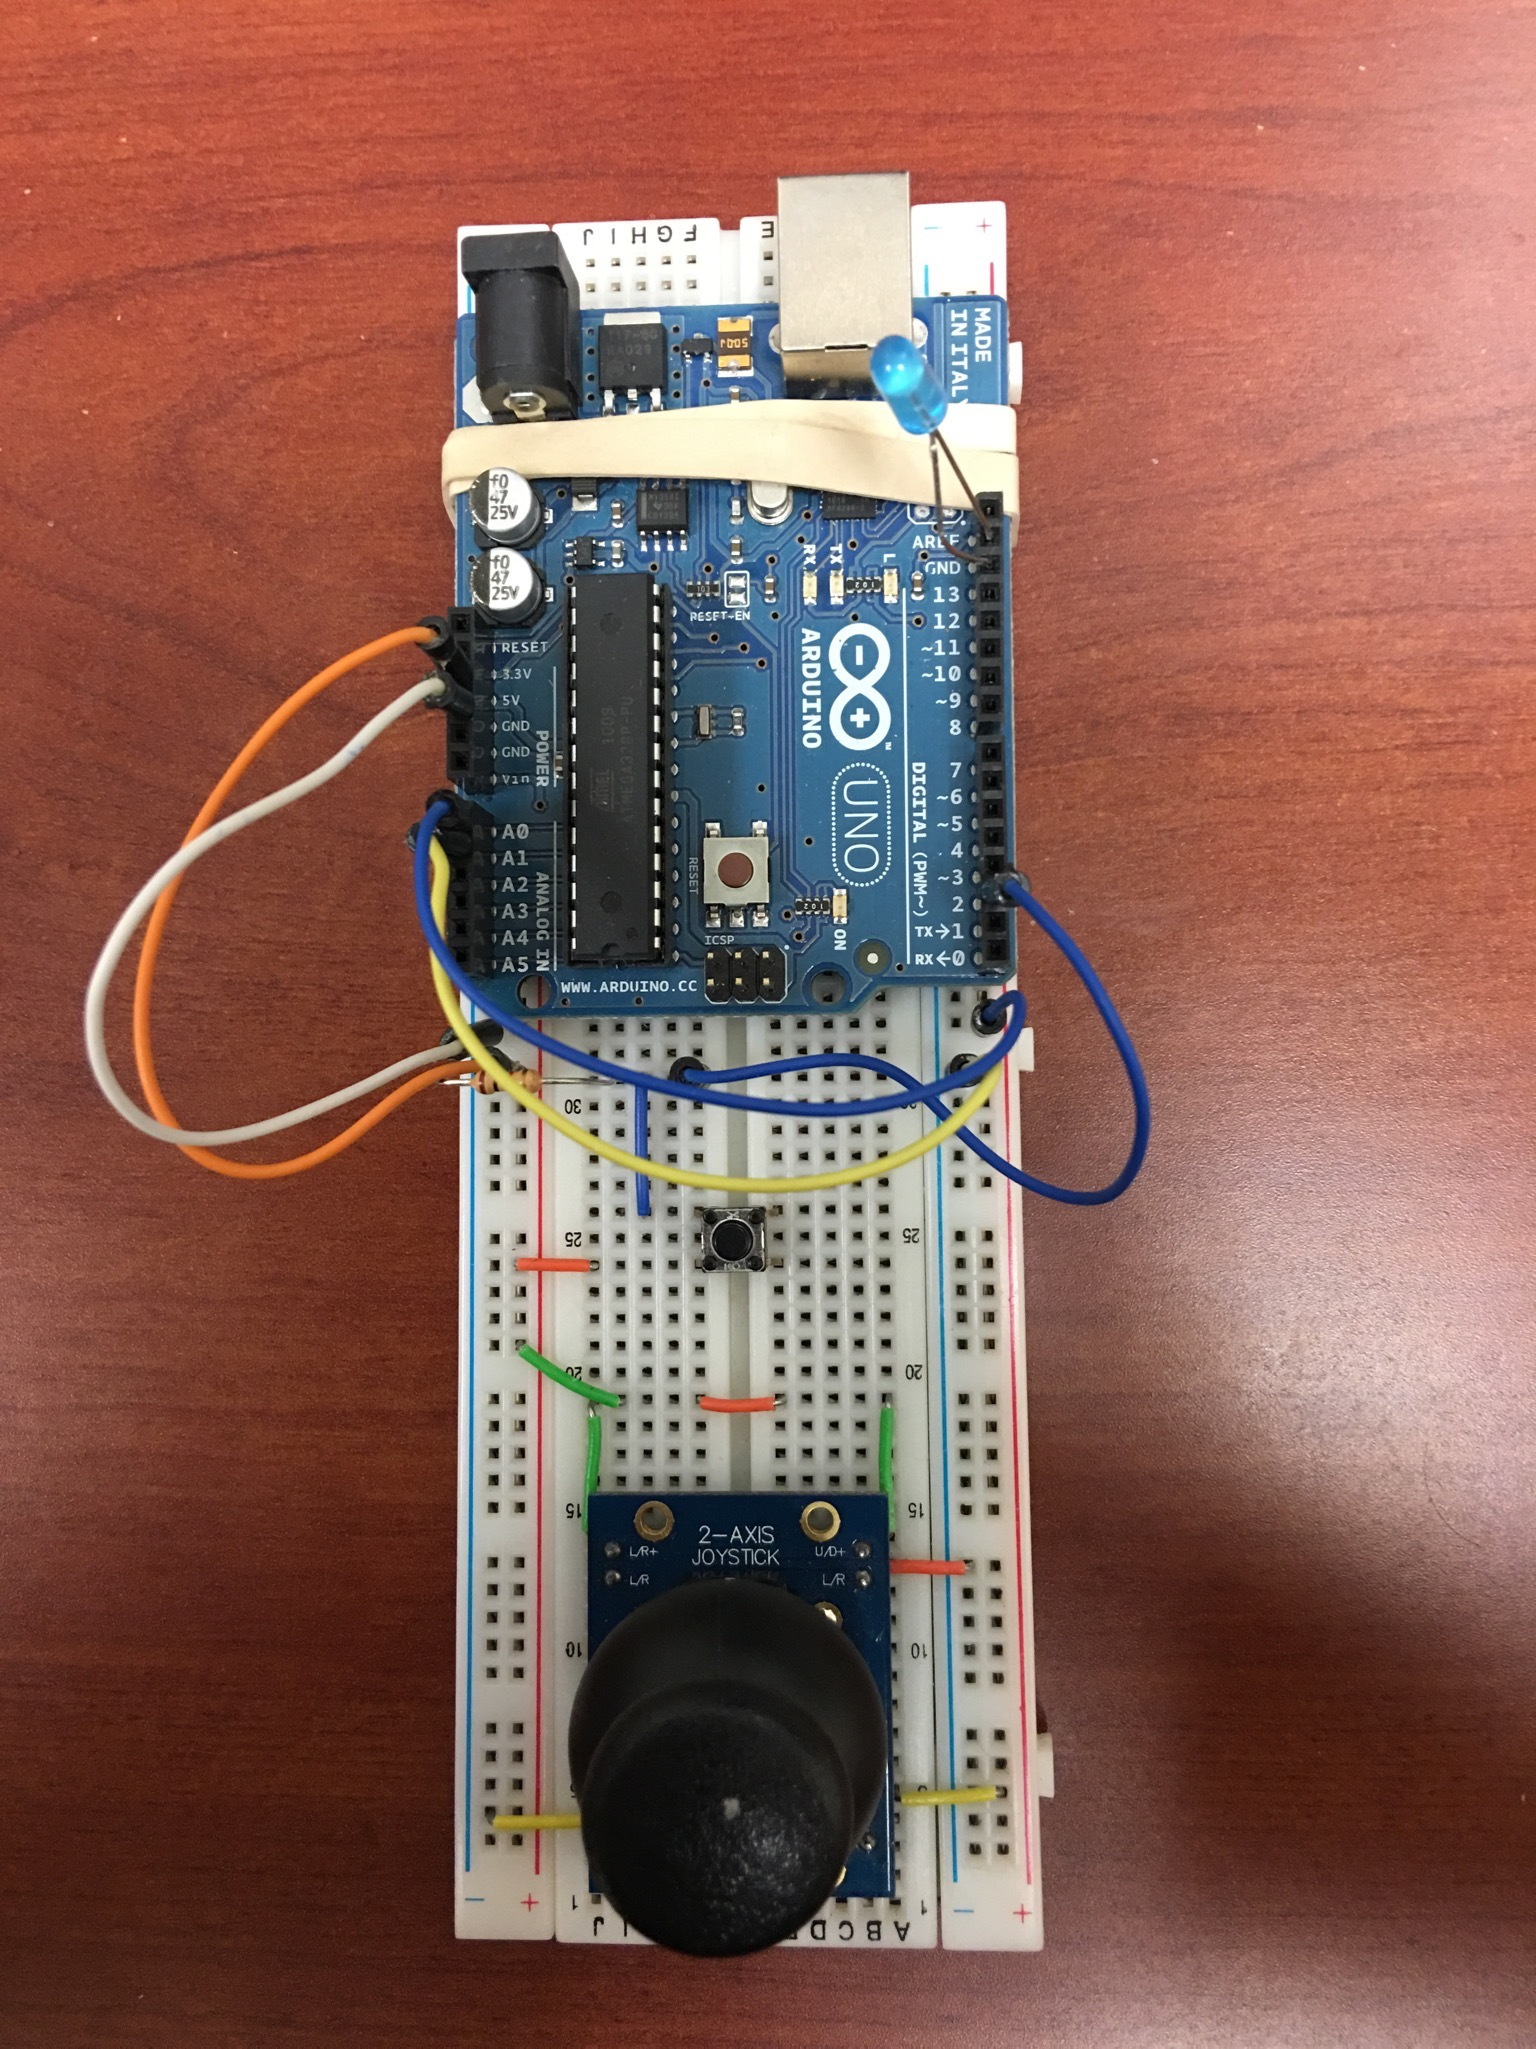
\includegraphics[scale=0.1]{arduino-gamecontroller/project}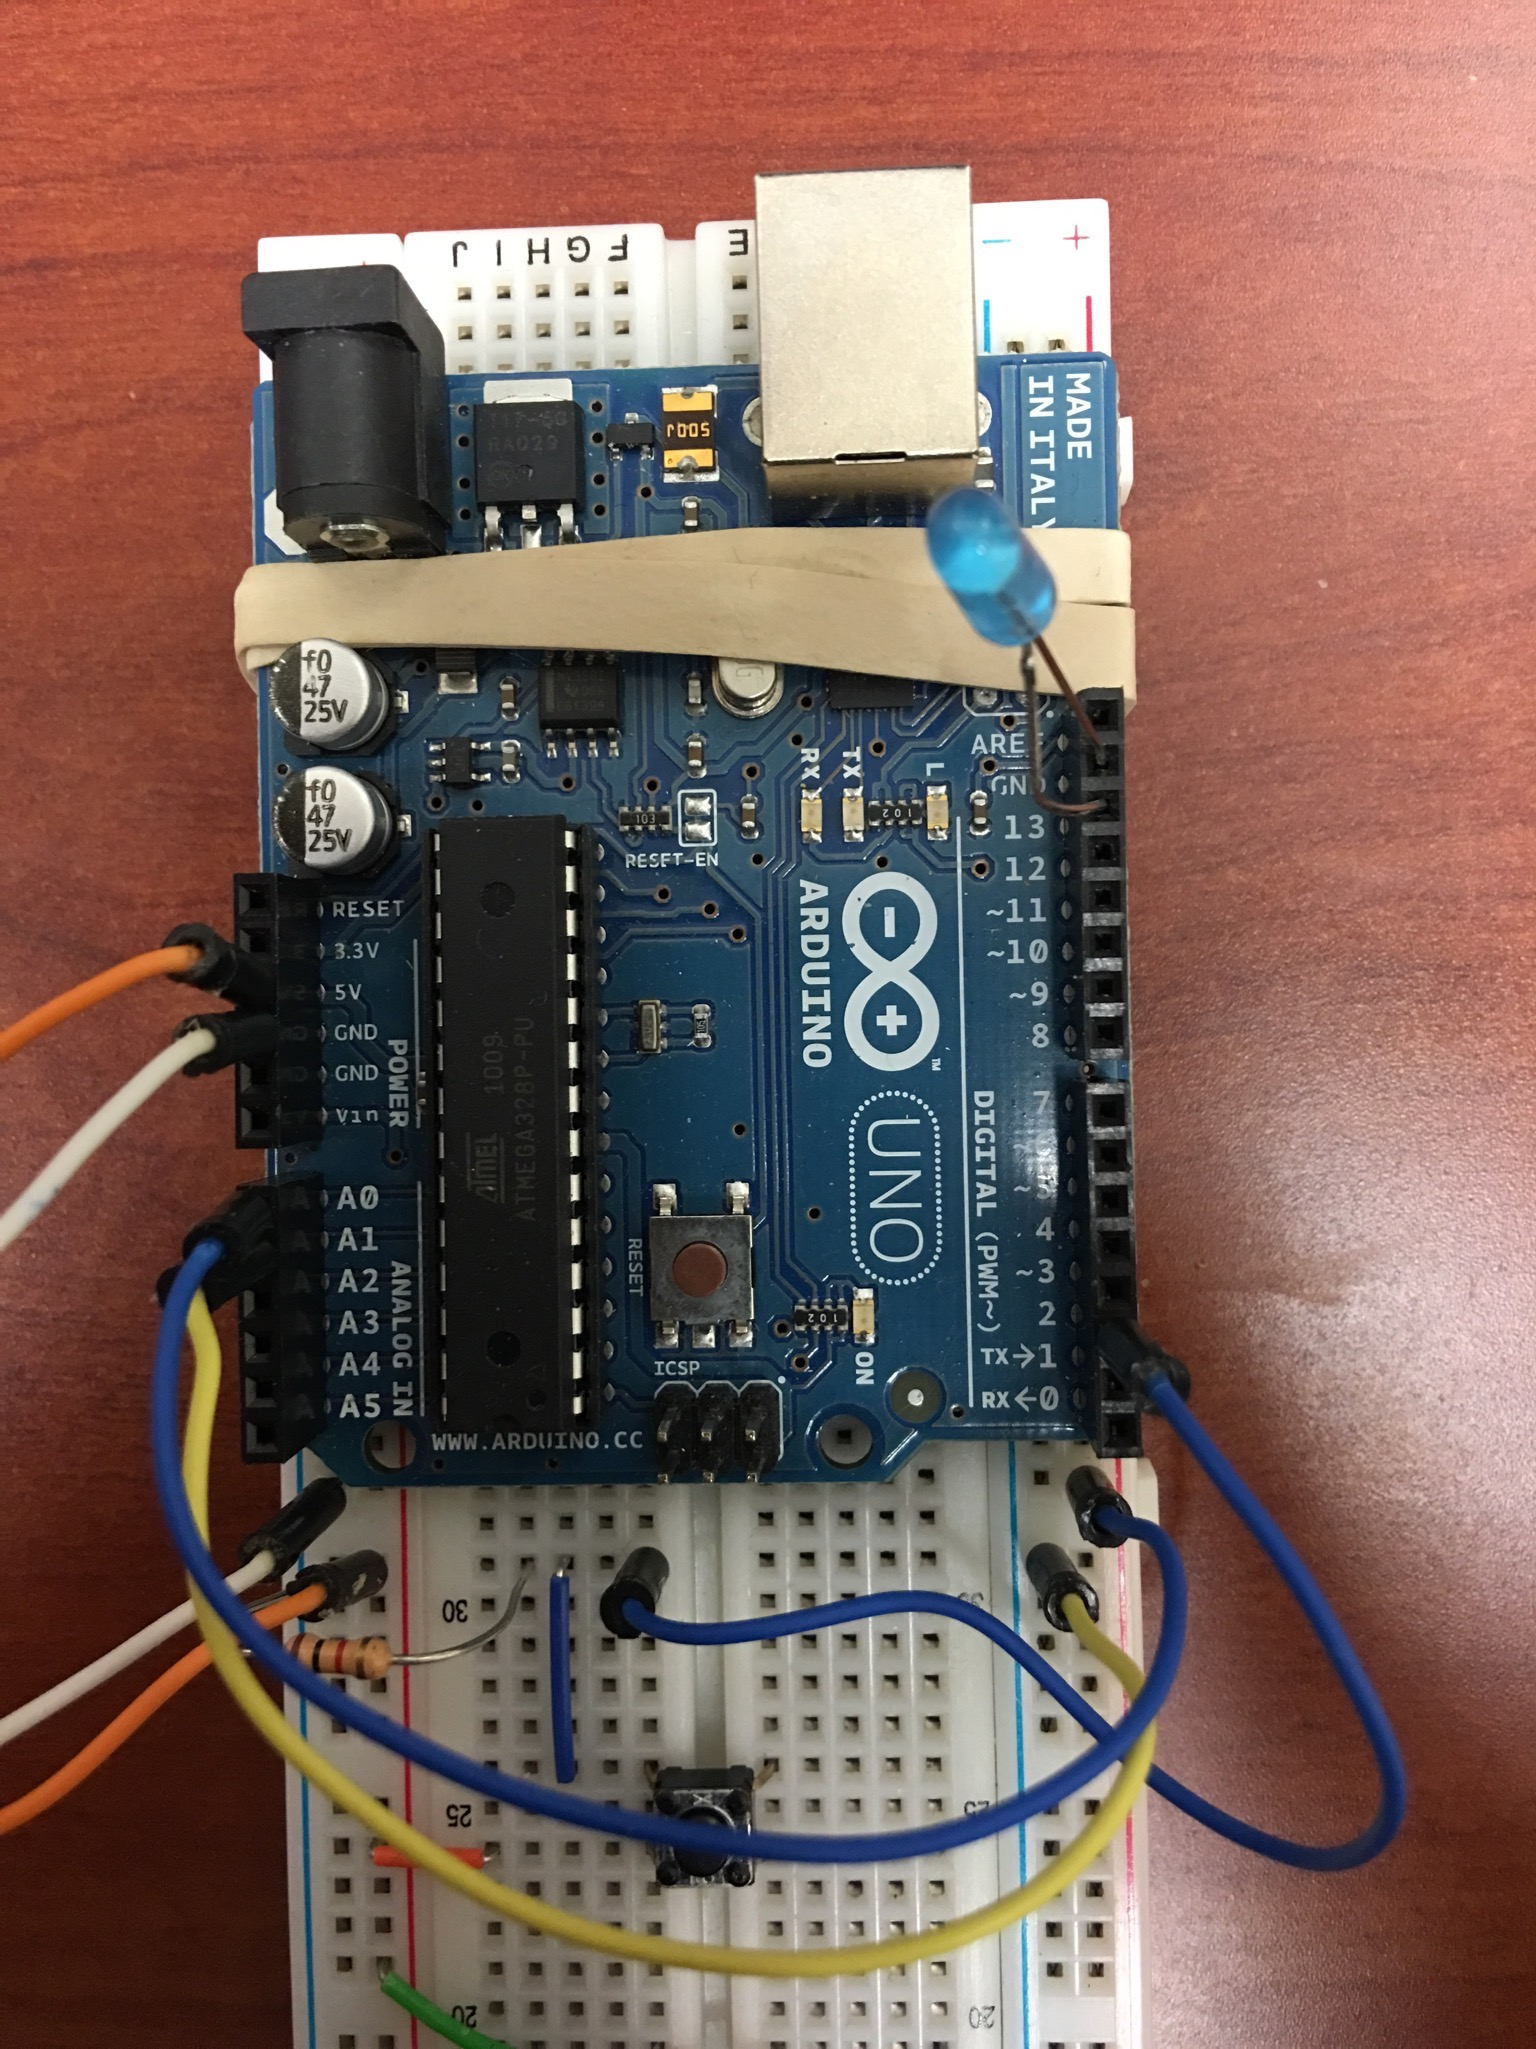
\includegraphics[scale=0.1]{arduino-gamecontroller/project-top}\\
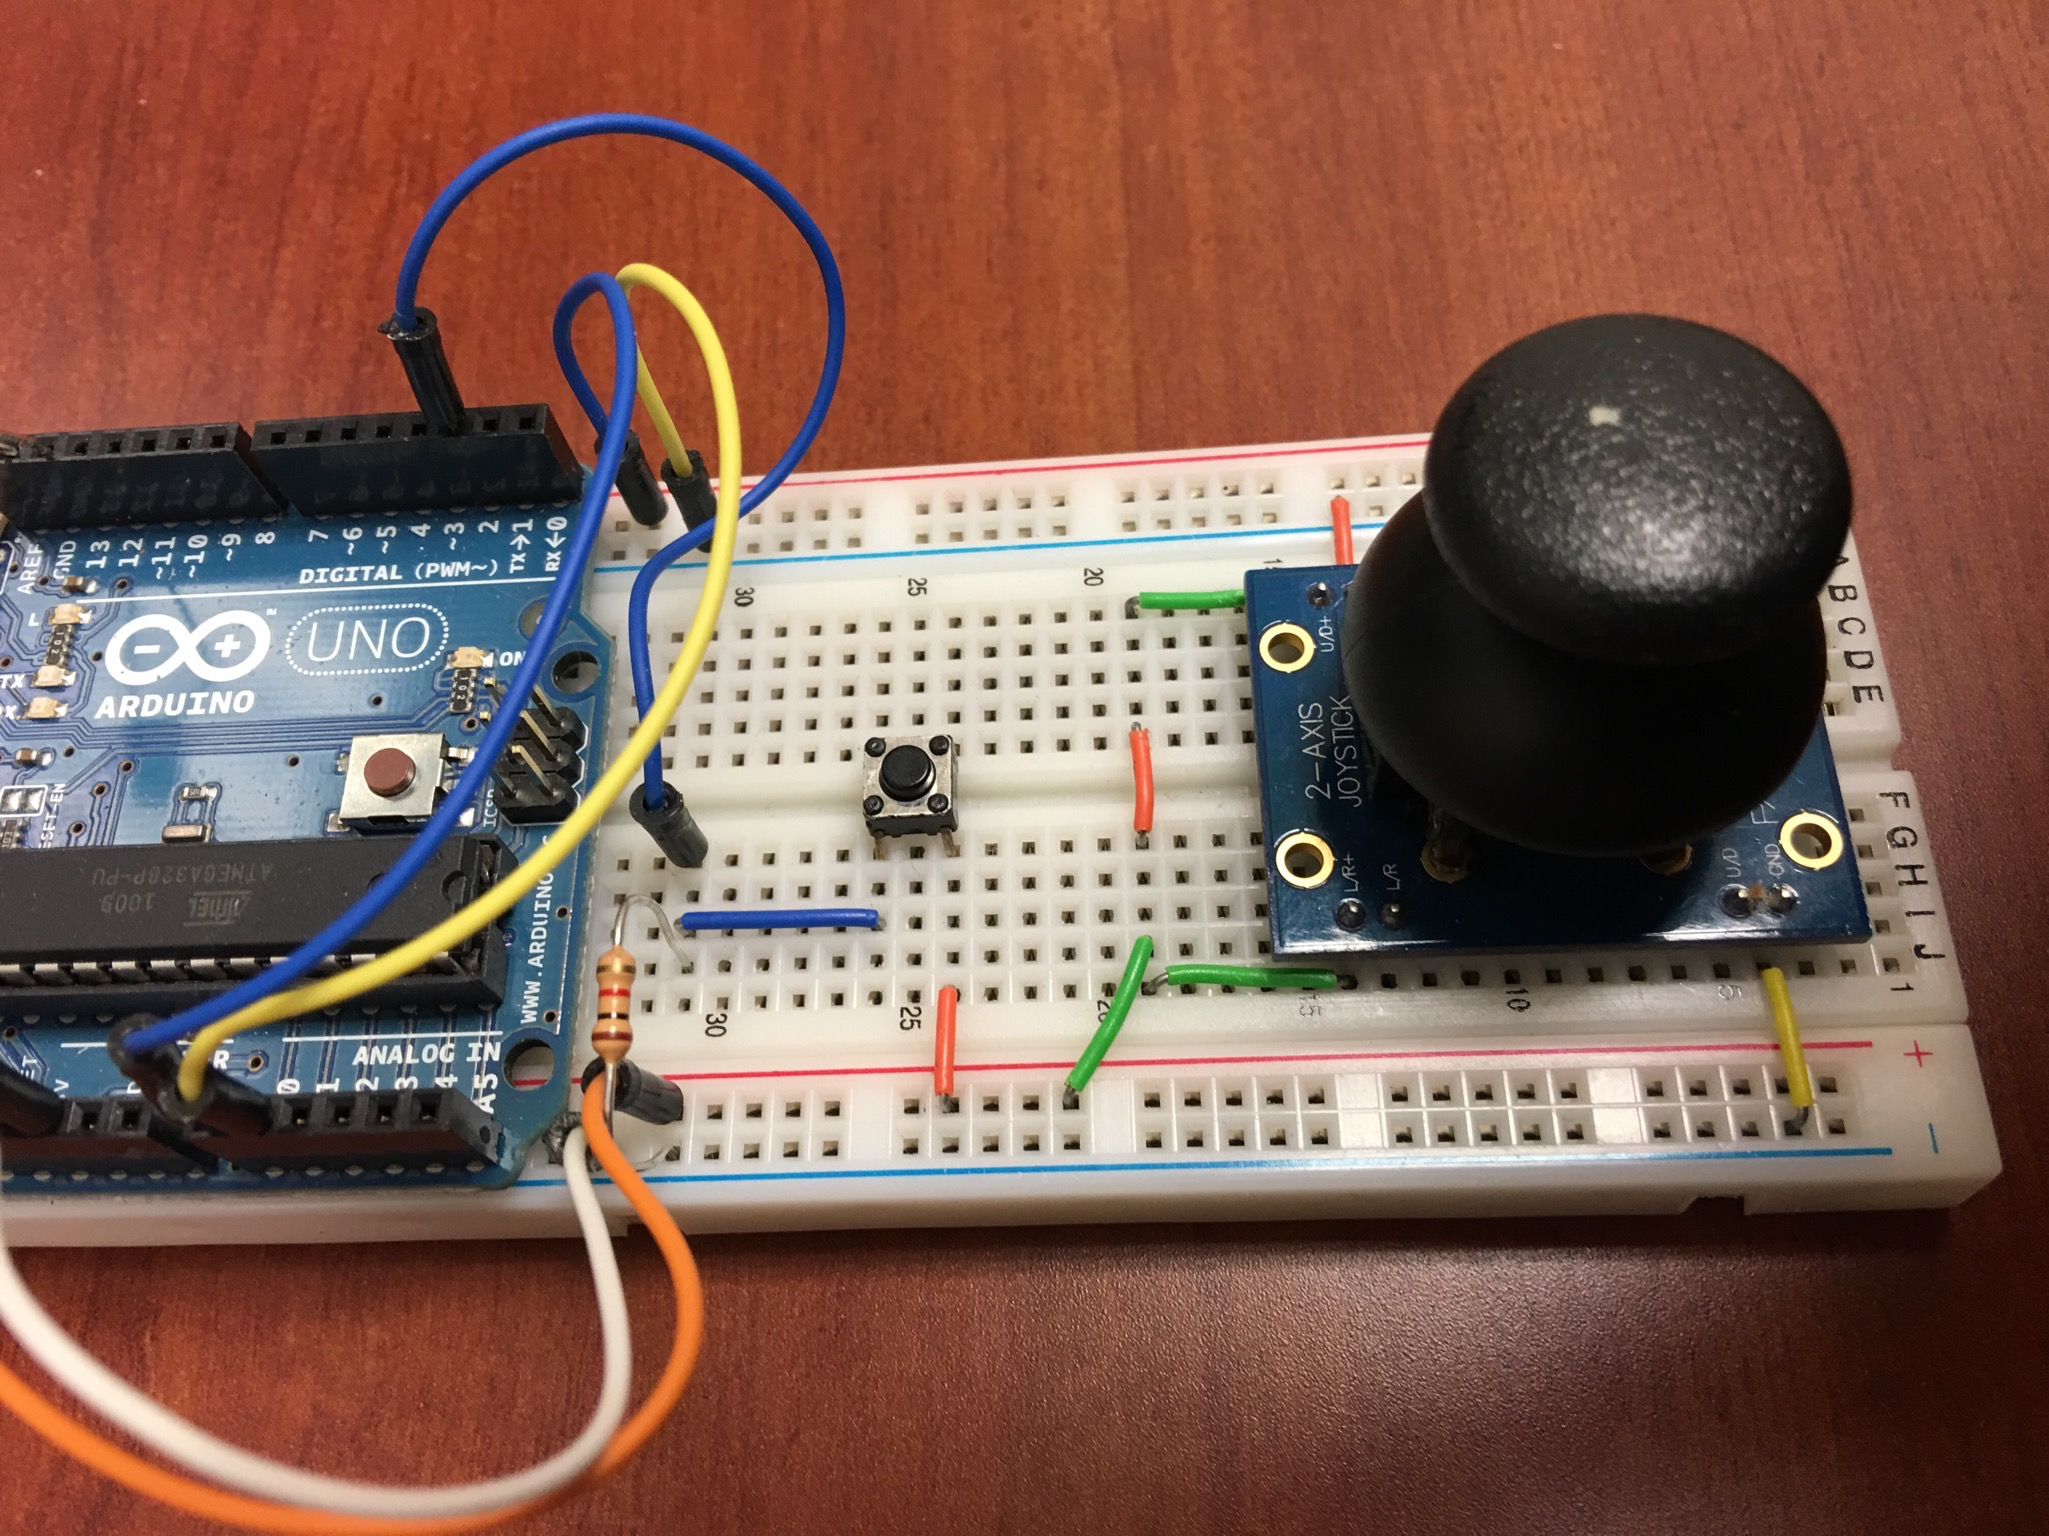
\includegraphics[scale=0.1]{arduino-gamecontroller/project-left}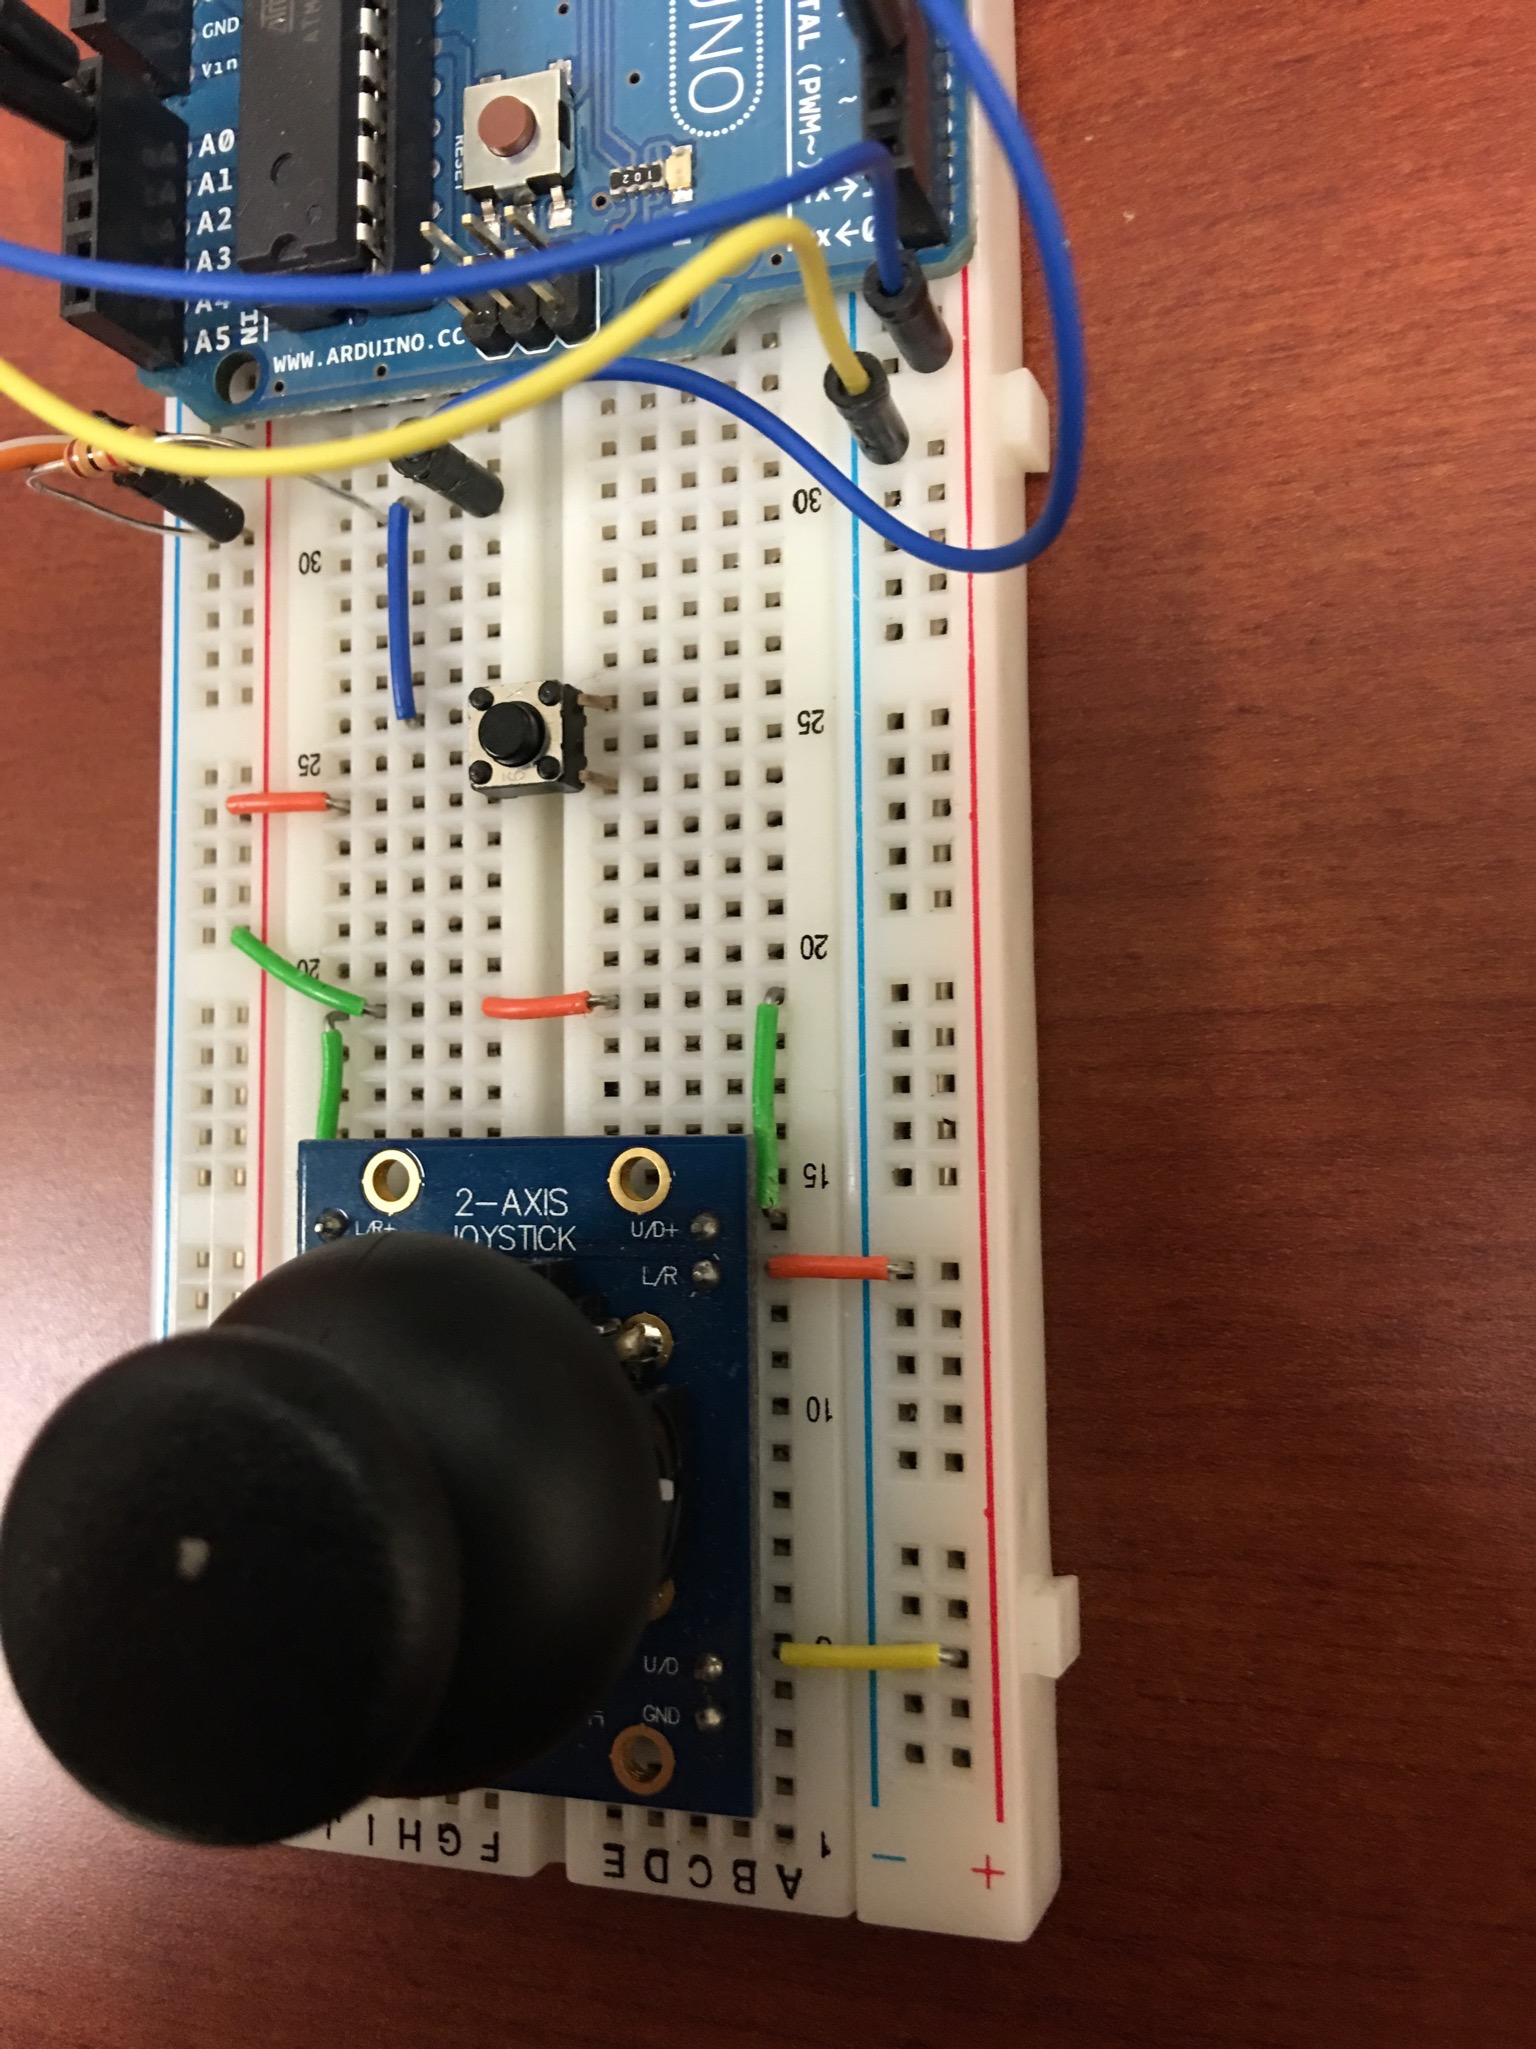
\includegraphics[scale=0.1]{arduino-gamecontroller/project-right}


\item Attach the Arduino to the breadboard with the rubber band.

\item Place the LED in pins 13 and GND. The LED has a long lead and a short lead. The long lead goes in pin 13 and the short lead goes in GND.

\item Run wires from GND (white wire) and +5 V (orange wire) pins on the left side of the Arduino to the -- and + columns on the left side of the breadboard, respectively. GND is wired to the -- column and 5 V is wired to the + column.

\item Run wires from pins A0 and A1 on the left side of the Arduino to the + and -- columns on the right side of the breadboard, respectively. A0 is wired to the +column an dA1 is wired to the -- column.

\item Attach the joystick to the breadboard. 

\item Wire the L/R+ and U/D+ pins on the joystick to +5 V (the + column on the left side of the breadboard).

\item Wire the GND pin on the joystick to GND (the -- column on the left side of the breadboard).

\item Wire the U/D pin on the joystick to pin A0 of the Arduino (the + column on the right side of the breadboard).

\item Wire the L/R pin on the joystick to pin A1 of the Arduino (the -- column on the right side of the breadboard).

\item The pushbutton switch, resistor, and the wire from pin 3 of the Arduino are not needed for the Lunar Lander game. You can add those parts later if you wish to fire bullets in Asteroids, for example.

\subsection*{Upload an Arduino program to the Arduino Uno}

We must upload a program to the Arduino that reads the voltage across each axis of the joystick and passed it to VPython when requested.

\item Download lunarLander.zip from our course web site. Here is the code.

\begin{arduinoblock}
#define UD A0
#define LR A1
int received;
char buffer[10];		  // input buffer
int N;			          // how many measurements to make
boolean done = false;


void setup() {
  Serial.begin(9600);
}

void loop() {
        received = 0;
    	buffer[received] = '\0';
    	done = false;
    
    	// Check input on serial line.
    	while (!done) {
    		if (Serial.available()) {	// Something is in the buffer
    			N = Serial.read();	// so get the number byte
    			done = true;
    		}
    	}
  
      int LRval = analogRead(LR);
      int UDval = analogRead(UD);
      Serial.print(LRval, DEC);
      Serial.print('\t');
      Serial.print(UDval, DEC);
      Serial.print('\n');
      delay(10);
}
\end{arduinoblock}

\item Open \code{lunarLander.ino}  with the Arduino software. The program looks like Figure \ref{arduino-gamecontroller/arduino-program}.

\scaledimage{arduino-gamecontroller/arduino-program}{An Arduino program running on the microprocessor.}{0.3}

\item Go to the \menu{Tools} menu and select \menu{Port}. One of these ports corresponds to the Arduino. Make sure  the correct one is checked, as shown in Figure \ref{arduino-gamecontroller/arduino-port}. This usually occurs by default.

\scaledimage{arduino-gamecontroller/arduino-port}{Select the serial port for your Arduiono}{0.3}

There are two important buttons in the top left corner of the menu bar. One is a checkmark and one is a right arrow, as shown in Figure \ref{arduino-gamecontroller/arduino-buttons}.

\scaledimage{arduino-gamecontroller/arduino-buttons}{Select the serial port for your Arduiono}{0.3}

\item The checkmark button is used to compile the Arduino program. It will tell you if there are any programming errors. Click the checkmark button to compile.

\item If there are no errors, then you are ready to upload the program to the microprocessor. Click the right arrow button to upload the program to the mircoprocessor.

The program should now be running on the microprocessor. It runs continuously in an infinite loop as long as it has power.

\subsection*{Running Lunar Lander with the Arduino game controller}

\item I have already created a Jupyter notebook that you can use as a template. Download the file \code{lunar-lander-nb.ipynb} from our course web site. Save the file (or move the file) into the folder where you stored your first Jupyter notebook file that you used to test the software.

\item  Go to the Jupyter browser window that shows your files and folders. Click on the file you just downloaded. It should open as a VPython notebook (as indicated in the top, right corner). 

\item Run the first cell. (It imports packages.)

\item The second cell has the code necessary to communicate with the Arduino. You need to get the serial port for your Arduino. Go to the Arduino software, click the \menu{Tools} menu and select \menu{Port}. Right down the name of the serial port that your Arduino is connected to. In your VPython notebook, edit the \code{port} variable to match the name of the port used by your Arduino. Mine is:

\begin{myvpython}
#serial port for the Arduino; get the name for the port from the Arduino software
port = '/dev/cu.usbmodem1a1221'
\end{myvpython}

Make sure the name of the port is contained within quotes since it is a string.

\item Run this cell and verify that there are no errors.

\item Run the third cell that contains the code for the game. You should see the lander, and you should be able to control it with your game controller.

%\scaledimage{arduino-gamecontroller/arduino-uno}{Arduino Uno microprocessor and breakout board.}{0.3}

\end{enumerate}

\pagebreak

\analysis

\begin{description}

\item[B] Complete this exercise and do the following.

\begin{enumerate}
	\item Upload a working notebook file produced at the end of this activity.
\end{enumerate}


\item[A] Do everything for {\bf B} with the following modifications and additions.

\begin{enumerate}
	\item Write a new game that uses the game controller and runs in a notebook.
\end{enumerate}




\end{description}

